\documentclass[12pt,a4paper]{article}
\usepackage{cmap} % Makes the PDF copiable. See http://tex.stackexchange.com/a/64198/25761
\usepackage[T1]{fontenc}
\usepackage[brazil]{babel}
\usepackage[utf8]{inputenc}
\usepackage{amsmath}
\usepackage{amsfonts}
\usepackage{amssymb}
\usepackage{amsthm}
\usepackage[usenames,svgnames,dvipsnames]{xcolor}
\usepackage{hyperref}
\usepackage{multicol}
\usepackage{graphicx}
\usepackage[margin=2cm]{geometry}
\usepackage{cancel}


\hypersetup{
    colorlinks = true,
    allcolors = {blue}
}

% TODO: Consider using exsheets
% http://linorg.usp.br/CTAN/macros/latex/contrib/exsheets/exsheets_en.pdf
%
% http://ctan.org/tex-archive/macros/latex/contrib/exercise/
% Options: answerdelayed,lastexercise,noanswer
\usepackage[answerdelayed,lastexercise]{exercise}

\addto\captionsbrazil{%
\def\listexercisename{Lista de exerc\'icios}%
\def\ExerciseName{Exerc\'icio}%
\def\AnswerName{Solu\c{c}\~ao do exerc\'icio}%
\def\ExerciseListName{Ex.}%
\def\AnswerListName{Solu\c{c}\~ao}%
\def\ExePartName{Parte}%
\def\ArticleOf{de\ }%
}

\renewcommand{\ExerciseHeaderTitle}{(\ExerciseTitle)\ }
\renewcommand{\ExerciseListHeader}{%\ExerciseHeaderDifficulty%
\textbf{%\ExerciseListName\
\ExerciseHeaderNB.\ %
%\ --- \
\ExerciseHeaderTitle}%
%\ExerciseHeaderOrigin
\ignorespaces}
\renewcommand{\AnswerListHeader}{\textbf{\ExerciseHeaderNB.\ (\AnswerListName)\ }}

\newcommand*\diff{\mathop{}\!\mathrm{d}}
\newcommand*\sen{\operatorname{sen}}

\newcommand*\op[1]{\overset{#1}{\rightarrow}}

\renewcommand{\theenumi}{\alph{enumi}}
\renewcommand\labelenumi{(\theenumi) }

\newcommand*\tipo{Prova II}
\newcommand*\turma{NEXM241-A}
\newcommand*\disciplina{CDI2001}
\newcommand*\eu{Helder G. G. de Lima}
\newcommand*\data{04/05/2024}

\author{\eu}
\title{\tipo - \disciplina}
\date{\data}

\begin{document}
\thispagestyle{empty}
\newgeometry{margin=2cm,bottom=0.5cm}
\begin{center}

\includegraphics[width=9.0cm]{marca} \\
\textbf{\tipo\ (\disciplina / \turma)} \\
Prof. \eu\footnote{
Este é um material de acesso livre distribuído sob os termos da licença \href{https://creativecommons.org/licenses/by-sa/4.0/deed.pt_BR}{Creative Commons BY-SA 4.0}}
\end{center}

\noindent Nome do(a) aluno(a): \underline{\hspace{9,7cm}} Data: \underline{\data}

%\section*{Instruções}
\begin{center}\fbox{
\begin{minipage}{14cm}

{\footnotesize
\begin{itemize}
\renewcommand{\theenumi}{\Roman{enumi}}
\item Identifique-se em todas as folhas.
\item Não é permitido o uso de calculadora.
\item Mantenha o celular e os demais equipamentos eletrônicos desligados durante a prova.
\item Justifique cada resposta com cálculos ou argumentos baseados na teoria estudada.
\item Resolva $5$ das $6$ questões (deixe claro que questão não deverá ser corrigida).
\end{itemize}
}

\end{minipage}
}
\end{center}

%\section*{Questões}
\begin{ExerciseList}
\Exercise[title={2,0}] Um sólido é obtido por meio da revolução da região delimitada por $f(x)=\sqrt{x \sen(x)}$, $x=-\pi/2$ e $x=\pi/2$ em torno do eixo $x$. Assinale a opção que indica o volume do sólido:
\begin{multicols}{5}
\begin{enumerate}
\item {\bf ( \ \ )} \ \ $\sqrt{2\pi}$
\item {\bf ( \ \ )} \ \ $-2\pi$
\item {\bf ( \ \ )} \ \ $\pi$
\item {\bf ( \ \ )} \ \ $2\pi$\label{volume}
\item {\bf ( \ \ )} \ \ $\pi^2$
\end{enumerate}
\end{multicols}
\Answer Alternativa (\ref{volume}): O volume é $V = 2\pi$. De fato, $x \sen(x) \geq 0$ em $[-\frac{\pi}{2}, \frac{\pi}{2}]$ e
\[
    V = \pi \int_{-\pi/2}^{\pi/2} \left[\sqrt{x \sen(x)}\right]^2 \diff{x}
      = \pi \int_{-\pi/2}^{\pi/2} x \sen(x) \diff{x}.
\]

\textbf{Solução 1}: Como $g(x) = x \sen(x)$ é par, sua integral definida de $-\frac{\pi}{2}$ a $\frac{\pi}{2}$ é o dobro da integral de $0$ a $\frac{\pi}{2}$:
\[
    V = 2 \pi \int_{0}^{\pi/2} x \sen(x) \diff{x}.
\]
Geometricamente, isso se deve à simetria do sólido em relação ao plano $yOz$:

\begin{center}
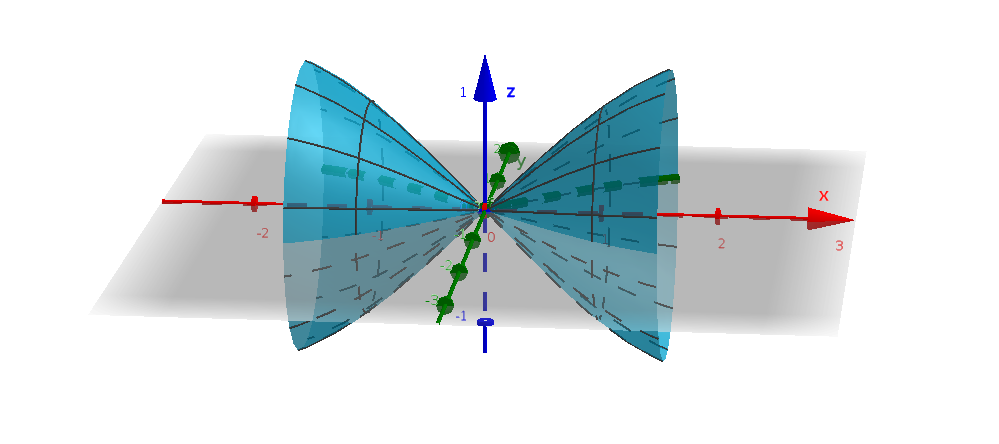
\includegraphics[width=12.0cm]{img/prova-2-nex-sólido-de-revolução.png}
\end{center}


Além disso, integrando por partes com $u=x$, $\diff{u} = \diff{x}$, $\diff{v} = \sen(x) \diff{x}$ e $v = -\cos(x)$, resulta:
\begin{align*}
    V & = 2\pi \left(\left(x \cdot(-\cos(x))\right)\bigg\rvert_{0}^{\pi/2} - \int_{0}^{\pi/2} -\cos(x) \diff{x}\right) \\
      & = 2\pi \left(\left(- x \cos(x) \right)\bigg\rvert_{0}^{\pi/2} + \left(\sen(x) \right)\bigg\rvert_{0}^{\pi/2}\right) \\
      & = 2\pi \left(\left[- (\pi/2) \cdot \cos(\pi/2) \right]-\left[- 0 \cdot \cos(0) \right] + \left[\sen(\pi/2) \right]-\left[\sen(0) \right]\right) \\
      & = 2\pi \left(0 - 0 + 1 - 0\right) = 2\pi.
\end{align*}

\textbf{Solução 2}: Também é possível calcular o volume sem usar a simetria do sólido. Neste caso,

\begin{align*}
    V & = \pi \int_{-\pi/2}^{\pi/2} x \sen(x) \diff{x}
        = \pi \left(\left(- x \cos(x) \right)\bigg\rvert_{-\pi/2}^{\pi/2} - \int_{-\pi/2}^{\pi/2} -\cos(x) \diff{x}\right) \\
      & = \pi \left(\left(- x \cos(x) + \sen(x) \right)\bigg\rvert_{-\pi/2}^{\pi/2}\right) \\
      & = \pi \left(\left[- (\pi/2) \cdot \cos(\pi/2) + \sen(\pi/2) \right] - \left[-(-\pi/2) \cdot \cos(-\pi/2) + \sen(-\pi/2) \right]\right) \\
      & = \pi \left([0 + 1] - [0 - 1 ]\right) = 2\pi.
\end{align*}


\Exercise[title={2,0}] Se $f(x,y) = \frac{y^2-x^4}{(y+x^2)\sqrt{y-x^2}}$ para $y > x^2$ e $f$ é contínua em $(-1, 1)$, quanto vale $f(-1, 1)$?
\Answer Da continuidade de $f$ em $(-1, 1)$ conclui-se que existe $\lim_{(x, y)\to (-1, 1)} f(x,y)$ e que esse limite é igual a $f(-1, 1)$.

\textbf{Solução 1}: Para determinar o valor desse limite, e consequentemente o valor de $f(-1, 1)$, observe que para todo $(x, y)$ satisfazendo $y > x^2$, tem-se:

\begin{align*}
f(x, y)
& = \frac{y^2-x^4}{(y+x^2)\sqrt{y-x^2}}
    = \frac{\cancel{(y+x^2)}(y-x^2)}{\cancel{(y+x^2)}\sqrt{y-x^2}}
    = \frac{(y-x^2)}{\sqrt{y-x^2}}\cdot\frac{\sqrt{y-x^2}}{\sqrt{y-x^2}} \\
& = \frac{\cancel{(y-x^2)} \sqrt{y-x^2}}{\cancel{y-x^2}}
    = \sqrt{y-x^2}.
\end{align*}

Portanto,
\[
  f(-1, 1)
  = \lim_{(x, y)\to (-1, 1)} f(x,y)
  = \lim_{(x, y)\to (-1, 1)} \sqrt{y-x^2}
  = \sqrt{\lim_{(x, y)\to (-1, 1)} y-x^2}
  = \sqrt{1-(-1)^2}
  = 0.
\]

\textbf{Solução 2}: Como $\lim_{(x, y)\to (-1, 1)} f(x,y)$ existe, o seu valor é o mesmo que o limite da função ao longo de qualquer caminho que passe pelo ponto $(-1, 1)$. Em particular, basta calcular o limite ao longo de uma reta, como $C_1 = \{(-1, y)\mid y \in \mathbb{R} \}$, e o resultado será igual a $f(-1, 1)$:

\begin{align*}
f(-1, 1)
& = \lim_{(x, y) \xrightarrow[C_1]{} (-1, 1)} \frac{y^2-x^4}{(y+x^2)\sqrt{y-x^2}}
  = \lim_{y\to 1} \frac{y^2-1}{(y+1)\sqrt{y-1}}
  = \lim_{y\to 1} \frac{y^2-1}{(y+1)\sqrt{y-1}} \cdot \frac{\sqrt{y-1}}{\sqrt{y-1}} \\
& = \lim_{y\to 1} \frac{(y^2-1)\sqrt{y-1}}{(y+1)(y-1)}
  = \lim_{y\to 1} \frac{\cancel{(y^2-1)}\sqrt{y-1}}{\cancel{y^2-1}}
  = \lim_{y\to 1} \sqrt{y-1}
  = \sqrt{1-1}
  = \sqrt{0}
  = 0.
\end{align*}

\Exercise[title={2,0}] Determine o plano tangente à superfície $z = 5\sqrt{x^2 + 9} + (y - 3)^2$ no ponto $A=(4, 6, 34)$.

\Answer Para calcular as derivadas parciais de primeira ordem de $f$, mantém-se uma variável livre e as demais constantes. Então, os valores de $\frac{\partial f}{\partial x}$ e $\frac{\partial f}{\partial y}$ em um ponto arbitrário $(x,y)\in\mathbb{R}^2$ são:
\[
\frac{\partial f}{\partial x}(x, y)
= \frac{\partial}{\partial x}\left(5\sqrt{x^2 + 9} + (y - 3)^2\right)
= \left(5\frac{2x}{2\sqrt{x^2 + 9}} + 0\right)
= \frac{5x}{\sqrt{x^2 + 9}}
\]
e
\[
\frac{\partial f}{\partial y}(x, y)
= \frac{\partial}{\partial y}\left(5\sqrt{x^2 + 9} + (y - 3)^2\right)
= 0 + 2(y-3)
= 2y-6.
\]
Em particular, no ponto $(4, 6)$, tem-se $\frac{\partial f}{\partial x}(4, 6) = \frac{5\cdot 4}{\sqrt{4^2 + 9}} = 4$ e $\frac{\partial f}{\partial y}(4, 6) = 2\cdot 6-6 = 6$. Assim, o plano tangente ao gráfico de $f$ em $A$ é:
\[
z-34 = 4(x-4) + 6(y-6),
\]
ou equivalentemente, $z = 4 x + 6 y - 18$, e sua representação geométrica é apresentada na figura a seguir:

\begin{center}
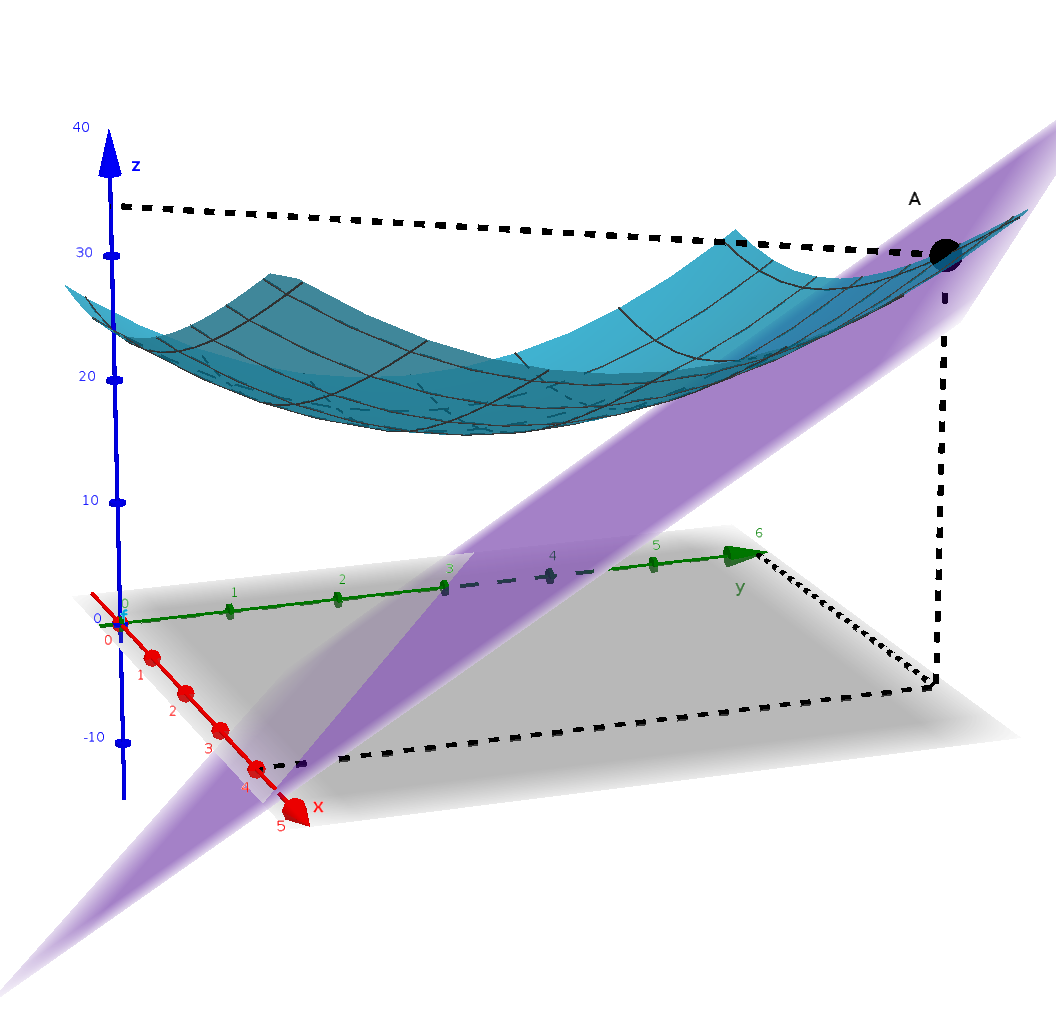
\includegraphics[width=8.0cm]{img/prova-2-nex-plano-tangente.png}
\end{center}


\Exercise[title={2,0}] Seja $f: \mathbb{R}^2 \setminus\{(0, 1)\} \to \mathbb{R}$ definida por $f(x,y) = \ln\left(x^2 + 4(y-1)^2\right)$.
\begin{enumerate}
\item (1,0 ponto) Descreva e represente geometricamente a curva de nível $k=0$ de $f$.
\item (1,0 ponto) Verifique que $\frac{\partial^2 f}{\partial y^2}(x, y) = -4 \frac{\partial^2 f}{\partial x^2}(x, y)$.
\end{enumerate}

\Answer
\begin{enumerate}
\item A curva de nível $k=0$ de $f$ é formada por pontos $(x, y) \in \mathbb{R}^2 \setminus\{(0, 1)\}$ tais que:
\[
    f(x, y) = \ln\left(x^2 + 4(y-1)^2\right) = 0
    \Leftrightarrow
    x^2 + 4(y-1)^2 = e^0
    \Leftrightarrow
    \frac{(x - 0)^2}{1^2} + \frac{(y-1)^2}{\left(\frac{1}{2}\right)^2} = 1.
\]
Sabe-se da geometria analítica que toda equação da forma $\frac{(x - x_0)^2}{a^2} + \frac{(y-y_0)^2}{b^2} = 1$ representa uma elipse com centro $(x_0, y_0)$ e eixos medindo $2a$ e $2b$. Portanto, a curva de nível é uma elipse com centro $(0, 1)$, eixo horizontal de comprimento $2$ e eixo vertical de comprimento $1$, conforme mostrado na figura a seguir:
\begin{center}
\includegraphics[width=6.0cm]{img/prova-2-nex-curva-de-nível-zero.pdf}
\end{center}
\item Mantendo $y$ fixo, e aplicando a regra da cadeia para funções de uma variável, obtém-se:
\[
\frac{\partial f}{\partial x}(x, y)
= \frac{\partial}{\partial x}\left(\ln\left(x^2 + 4(y-1)^2\right)\right)
= \frac{2x}{x^2 + 4(y-1)^2}.
\]
Além disso, fixando $x$ e aplicando a regra da cadeia para funções de uma variável, obtém-se:
\[
\frac{\partial f}{\partial y}(x, y)
= \frac{\partial}{\partial y}\left(\ln\left(x^2 + 4(y-1)^2\right)\right)
=\frac{8(y-1)}{x^2 + 4(y-1)^2}.
\]
Consequentemente, as derivadas de segunda ordem $\frac{\partial^2 f}{\partial x^2}$ e $\frac{\partial^2 f}{\partial y^2}$ em um ponto $(x,y)$ são:
\begin{align*}
\frac{\partial^2 f}{\partial x^2}(x, y)
  = \frac{\partial}{\partial x}\left(\frac{2x}{x^2 + 4(y-1)^2}\right)
  = \frac{2\cdot(x^2 + 4(y-1)^2) - 2x \cdot 2x}{x^2 + 4(y-1)^2}
  = \frac{-2 x^2 + 8(y-1)^2}{x^2 + 4(y-1)^2}
\end{align*}
e
\begin{align*}
\frac{\partial^2 f}{\partial y^2}(x, y)
  & = \frac{\partial}{\partial y}\left(\frac{8(y-1)}{x^2 + 4(y-1)^2}\right)
    = \frac{8\cdot(x^2 + 4(y-1)^2) - 8(y-1)\cdot 8(y-1)}{x^2 + 4(y-1)^2} \\
  & = \frac{8x^2 - 32(y-1)^2}{x^2 + 4(y-1)^2}
    = -4 \frac{\partial^2 f}{\partial x^2}(x, y).
\end{align*}
\end{enumerate}


\Exercise[title={2,0}] Se $z=f(12x-8y, 4y-6x)$ e $f$ tem derivadas parciais contínuas, calcule $2\frac{\partial z}{\partial x} + 3\frac{\partial z}{\partial y}$.
\Answer Seja $z=f(u, v)$ com $u = u(x,y) = 12x - 8y$ e $v = v(x,y) = 4y - 6x$. Por hipótese, as derivadas parciais $\frac{\partial f}{\partial u}$ e $\frac{\partial f}{\partial v}$ existem e são contínuas. Então, pela regra da cadeia:
\[
  \frac{\partial z}{\partial x}
  = \frac{\partial f}{\partial u} \frac{\partial u}{\partial x}
    + \frac{\partial f}{\partial v} \frac{\partial v}{\partial x}
  = \frac{\partial f}{\partial u} 12
    + \frac{\partial f}{\partial v} (-6)
\]
e
\[
  \frac{\partial z}{\partial y}
  = \frac{\partial f}{\partial u} \frac{\partial u}{\partial y}
    + \frac{\partial f}{\partial v} \frac{\partial v}{\partial y}
  = \frac{\partial f}{\partial u} (-8)
    + \frac{\partial f}{\partial v} 4.
\]
Então
\[
  2\frac{\partial z}{\partial x} + 3\frac{\partial z}{\partial y}
  = 2\left[\frac{\partial f}{\partial u} 12
    + \frac{\partial f}{\partial v} (-6)\right]
    + 3\left[\frac{\partial f}{\partial u} (-8)
    + \frac{\partial f}{\partial v} 4\right]
  = 24 \frac{\partial f}{\partial u}
    - 12 \frac{\partial f}{\partial v}
    - 24\frac{\partial f}{\partial u}
    + 12 \frac{\partial f}{\partial v}
  = 0.
\]


\Exercise[title={2,0}] Para cada item abaixo, diga se é verdadeiro (V) ou falso (F).

\emph{Observação 1.} Não é necessário justificar esta questão.

\emph{Observação 2.} Cada item marcado errado anula a pontuação de um item marcado corretamente. Você tem a opção de deixar o item em branco e, nesse caso, você nem ganha e nem perde pontos.


\begin{enumerate}
\item (0,5 ponto) {\bf ( \ \ )} \ O sólido obtido pela rotação de $f:[a,b]\to\mathbb{R}$ em torno da reta $y = \pi$ tem volume $V = \pi \int_a^b \left[f(x)-\pi\right]^2 \diff{x}$.
\item (0,5 ponto) {\bf ( \ \ )} \ Se o limite de $f(x,y)$ ao longo de toda reta que passa por $(0,0)$ for $1$, então o limite de $f$ existe e $\lim_{(x,y)\to(0,0)} f(x,y) = 1$.
\item (0,5 ponto) {\bf ( \ \ )} \ $\lim_{(x,y)\to(0,0)} \cos\left(\sqrt[5]{\frac{2xy^2+3x^2y}{xy}}\right) = 1$.
\item (0,5 ponto) {\bf ( \ \ )} \ Se $h(x, y) = \frac{x^2}{2} + xy + \frac{y^2}{2}$ então $\frac{\partial h}{\partial x}(x, y) = \frac{\partial h}{\partial y}(x, y)$.
\end{enumerate}

\Answer \begin{enumerate}
\item \textbf{Verdadeiro}. Em geral, o sólido obtido pela rotação de $f:[a,b]\to\mathbb{R}$ em torno de uma reta $y = c$ tem volume $V = \pi \int_a^b \left[f(x)-c\right]^2 \diff{x}$.
\item \textbf{Falso}. É preciso que o limite seja $1$ ao longo de todos os caminhos que passam por $(0, 0)$, não apenas ao longo de retas.
\item \textbf{Verdadeiro}. Como
\[
\lim_{(x, y)\to(0, 0)} \frac{2xy^2 + 3x^2y}{xy}
= \lim_{(x, y)\to(0, 0)} \frac{2xy^2}{xy} + \frac{3x^2y}{xy}
= \lim_{(x, y)\to(0, 0)} 3x + 2y
= 3 \cdot 0 + 2 \cdot 0
= 0,
\]
e a função $g:\mathbb{R} \to \mathbb{R}$ definida por $g(x) = \cos\left(\sqrt[5]{x}\right)$ é contínua em $x = 0$, tem-se:
\[
\lim_{(x,y)\to(0,0)} \cos\left(\sqrt[5]{\frac{2xy^2+3x^2y}{xy}}\right)
= \cos\left(\sqrt[5]{ \lim_{(x,y)\to(0,0)} \frac{2xy^2+3x^2y}{xy}}\right)
= \cos\left(\sqrt[5]{0}\right)
= 1.
\]
\item \textbf{Verdadeiro}. De fato, mantendo $y$ constante obtém-se
\[
\frac{\partial h}{\partial x}(x, y)
= \frac{\partial}{\partial x}\left( \frac{x^2}{2} + xy + \frac{y^2}{2} \right)
= \frac{2x}{2} + y + 0
= x + y
\]
e mantendo $x$ constante obtém-se
\[
\frac{\partial h}{\partial y}(x, y)
= \frac{\partial}{\partial y}\left( \frac{x^2}{2} + xy + \frac{y^2}{2} \right)
= 0 + x + \frac{2y}{2}
= x + y.
\]
\end{enumerate}
\end{ExerciseList}

\begin{center}
BOA PROVA!
\end{center}

\newpage
\restoregeometry
\section*{Respostas}
\shipoutAnswer
\end{document}
